\documentclass{standalone}
\usepackage{tikz}
\usetikzlibrary{patterns, positioning}


\begin{document}
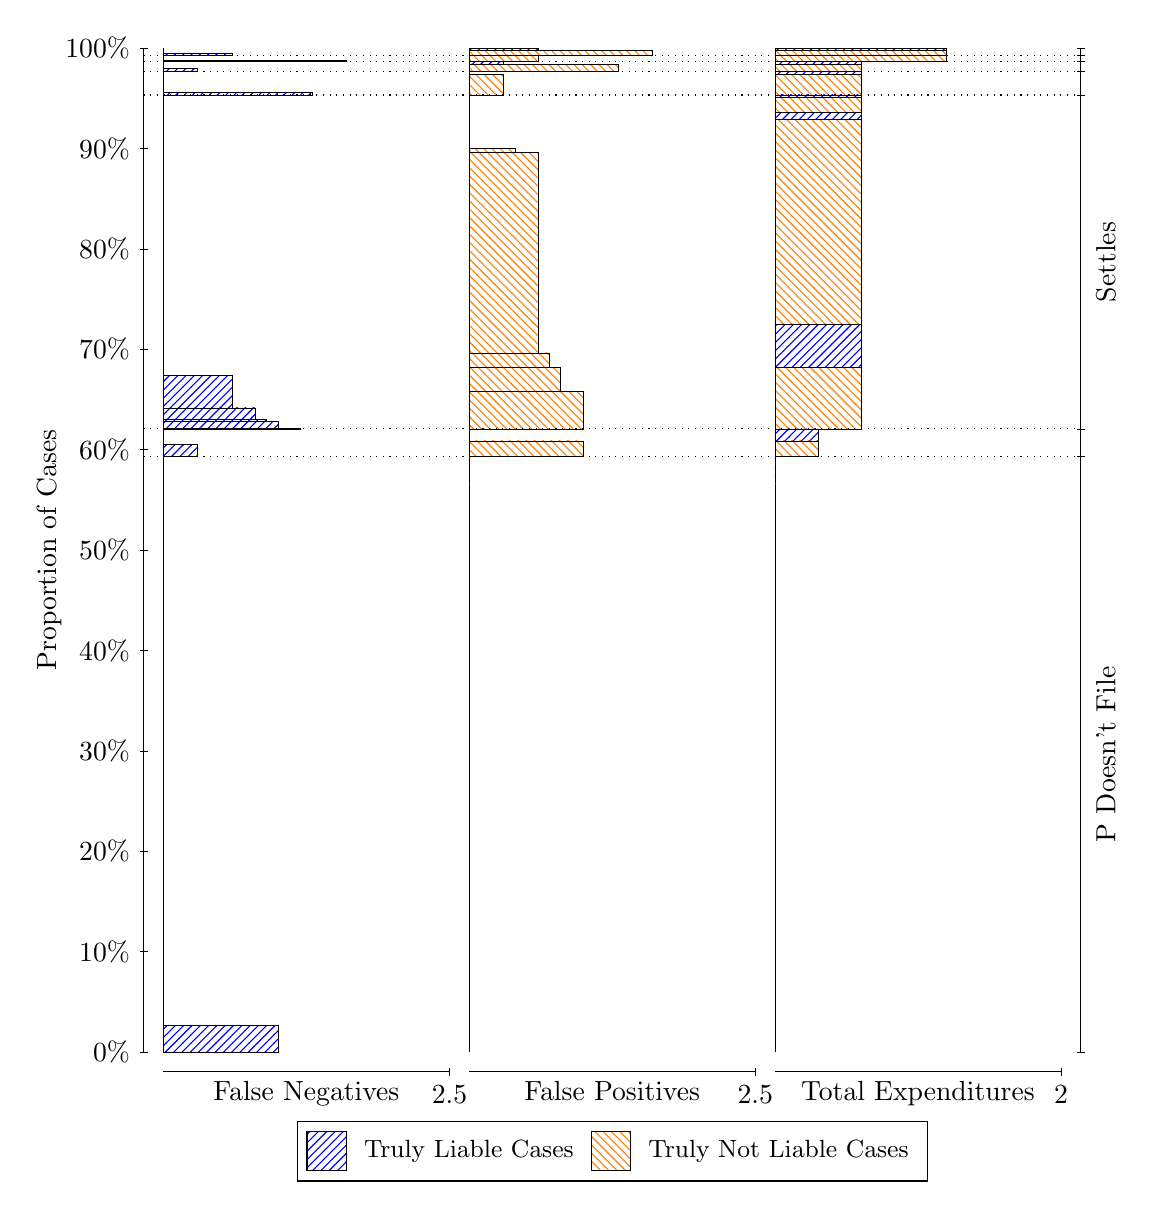
\begin{tikzpicture}
\draw[black, very thin] (1.5,1.75) -- (1.5,14.5);
\node[rotate=90, text=black, anchor=center] at (0.3, 8.125) {Proportion of Cases};
\draw[black, very thin] (1.45,1.75) -- (1.55,1.75);
\node[text=black, anchor=east] at (1.45, 1.75) {0\%};
\draw[black, very thin] (1.45,3.025) -- (1.55,3.025);
\node[text=black, anchor=east] at (1.45, 3.025) {10\%};
\draw[black, very thin] (1.45,4.3) -- (1.55,4.3);
\node[text=black, anchor=east] at (1.45, 4.3) {20\%};
\draw[black, very thin] (1.45,5.575) -- (1.55,5.575);
\node[text=black, anchor=east] at (1.45, 5.575) {30\%};
\draw[black, very thin] (1.45,6.85) -- (1.55,6.85);
\node[text=black, anchor=east] at (1.45, 6.85) {40\%};
\draw[black, very thin] (1.45,8.125) -- (1.55,8.125);
\node[text=black, anchor=east] at (1.45, 8.125) {50\%};
\draw[black, very thin] (1.45,9.4) -- (1.55,9.4);
\node[text=black, anchor=east] at (1.45, 9.4) {60\%};
\draw[black, very thin] (1.45,10.675) -- (1.55,10.675);
\node[text=black, anchor=east] at (1.45, 10.675) {70\%};
\draw[black, very thin] (1.45,11.95) -- (1.55,11.95);
\node[text=black, anchor=east] at (1.45, 11.95) {80\%};
\draw[black, very thin] (1.45,13.225) -- (1.55,13.225);
\node[text=black, anchor=east] at (1.45, 13.225) {90\%};
\draw[black, very thin] (1.45,14.5) -- (1.55,14.5);
\node[text=black, anchor=east] at (1.45, 14.5) {100\%};

\draw[black, very thin] (13.4,1.75) -- (13.4,14.5);
\draw[black, very thin] (13.35,1.75) -- (13.45,1.75);
\node[anchor=west] at (13.35, 1.75) {};
\draw[black, very thin] (13.35,9.313) -- (13.45,9.313);
\node[anchor=west] at (13.35, 9.313) {};
\draw[black, very thin] (13.35,9.6626) -- (13.45,9.6626);
\node[anchor=west] at (13.35, 9.6626) {};
\draw[black, very thin] (13.35,13.904) -- (13.45,13.904);
\node[anchor=west] at (13.35, 13.904) {};
\draw[black, very thin] (13.35,14.204) -- (13.45,14.204);
\node[anchor=west] at (13.35, 14.204) {};
\draw[black, very thin] (13.35,14.331) -- (13.45,14.331);
\node[anchor=west] at (13.35, 14.331) {};
\draw[black, very thin] (13.35,14.409) -- (13.45,14.409);
\node[anchor=west] at (13.35, 14.409) {};
\draw[black, very thin] (13.35,14.5) -- (13.45,14.5);
\node[anchor=west] at (13.35, 14.5) {};

\draw[black, very thin, pattern color=blue, pattern=north east lines] (1.75,1.75) rectangle (3.2033,2.0919);
\draw[black, very thin, pattern color=orange, pattern=north west lines] (1.75,2.0919) rectangle (1.75,9.313);
\draw[black, very thin, pattern color=blue, pattern=north east lines] (1.75,9.313) rectangle (2.186,9.4642);
\draw[black, very thin, pattern color=orange, pattern=north west lines] (1.75,9.4642) rectangle (1.75,9.6626);
\draw[black, very thin, pattern color=blue, pattern=north east lines] (1.75,9.6626) rectangle (3.494,9.6689);
\draw[black, very thin, pattern color=blue, pattern=north east lines] (1.75,9.6689) rectangle (3.2033,9.755);
\draw[black, very thin, pattern color=blue, pattern=north east lines] (1.75,9.755) rectangle (3.058,9.7877);
\draw[black, very thin, pattern color=blue, pattern=north east lines] (1.75,9.7877) rectangle (2.9127,9.9311);
\draw[black, very thin, pattern color=blue, pattern=north east lines] (1.75,9.9311) rectangle (2.622,10.338);
\draw[black, very thin, pattern color=orange, pattern=north west lines] (1.75,10.338) rectangle (1.75,13.904);
\draw[black, very thin, pattern color=blue, pattern=north east lines] (1.75,13.904) rectangle (3.6393,13.94);
\draw[black, very thin, pattern color=orange, pattern=north west lines] (1.75,13.94) rectangle (1.75,14.204);
\draw[black, very thin, pattern color=blue, pattern=north east lines] (1.75,14.204) rectangle (2.186,14.242);
\draw[black, very thin, pattern color=orange, pattern=north west lines] (1.75,14.242) rectangle (1.75,14.331);
\draw[black, very thin, pattern color=blue, pattern=north east lines] (1.75,14.331) rectangle (4.0753,14.339);
\draw[black, very thin, pattern color=orange, pattern=north west lines] (1.75,14.339) rectangle (1.75,14.409);
\draw[black, very thin, pattern color=blue, pattern=north east lines] (1.75,14.409) rectangle (2.622,14.436);
\draw[black, very thin, pattern color=orange, pattern=north west lines] (1.75,14.436) rectangle (1.75,14.5);
\draw[black, very thin, pattern color=orange, pattern=north west lines] (5.6333,1.75) rectangle (5.6333,8.9711);
\draw[black, very thin, pattern color=blue, pattern=north east lines] (5.6333,8.9711) rectangle (5.6333,9.313);
\draw[black, very thin, pattern color=orange, pattern=north west lines] (5.6333,9.313) rectangle (7.0867,9.5114);
\draw[black, very thin, pattern color=blue, pattern=north east lines] (5.6333,9.5114) rectangle (5.6333,9.6626);
\draw[black, very thin, pattern color=orange, pattern=north west lines] (5.6333,9.6626) rectangle (7.0867,10.138);
\draw[black, very thin, pattern color=orange, pattern=north west lines] (5.6333,10.138) rectangle (6.796,10.442);
\draw[black, very thin, pattern color=orange, pattern=north west lines] (5.6333,10.442) rectangle (6.6507,10.627);
\draw[black, very thin, pattern color=orange, pattern=north west lines] (5.6333,10.627) rectangle (6.5053,13.175);
\draw[black, very thin, pattern color=orange, pattern=north west lines] (5.6333,13.175) rectangle (6.2147,13.229);
\draw[black, very thin, pattern color=blue, pattern=north east lines] (5.6333,13.229) rectangle (5.6333,13.904);
\draw[black, very thin, pattern color=orange, pattern=north west lines] (5.6333,13.904) rectangle (6.0693,14.168);
\draw[black, very thin, pattern color=blue, pattern=north east lines] (5.6333,14.168) rectangle (5.6333,14.204);
\draw[black, very thin, pattern color=orange, pattern=north west lines] (5.6333,14.204) rectangle (7.5227,14.294);
\draw[black, very thin, pattern color=blue, pattern=north east lines] (5.6333,14.294) rectangle (6.0693,14.331);
\draw[black, very thin, pattern color=orange, pattern=north west lines] (5.6333,14.331) rectangle (6.5053,14.402);
\draw[black, very thin, pattern color=blue, pattern=north east lines] (5.6333,14.402) rectangle (5.6333,14.409);
\draw[black, very thin, pattern color=orange, pattern=north west lines] (5.6333,14.409) rectangle (7.9587,14.474);
\draw[black, very thin, pattern color=blue, pattern=north east lines] (5.6333,14.474) rectangle (6.5053,14.5);
\draw[black, very thin, pattern color=orange, pattern=north west lines] (9.5167,1.75) rectangle (9.5167,8.9711);
\draw[black, very thin, pattern color=blue, pattern=north east lines] (9.5167,8.9711) rectangle (9.5167,9.313);
\draw[black, very thin, pattern color=orange, pattern=north west lines] (9.5167,9.313) rectangle (10.062,9.5114);
\draw[black, very thin, pattern color=blue, pattern=north east lines] (9.5167,9.5114) rectangle (10.062,9.6626);
\draw[black, very thin, pattern color=orange, pattern=north west lines] (9.5167,9.6626) rectangle (10.607,10.442);
\draw[black, very thin, pattern color=blue, pattern=north east lines] (9.5167,10.442) rectangle (10.607,10.992);
\draw[black, very thin, pattern color=orange, pattern=north west lines] (9.5167,10.992) rectangle (10.607,13.595);
\draw[black, very thin, pattern color=blue, pattern=north east lines] (9.5167,13.595) rectangle (10.607,13.687);
\draw[black, very thin, pattern color=orange, pattern=north west lines] (9.5167,13.687) rectangle (10.607,13.872);
\draw[black, very thin, pattern color=blue, pattern=north east lines] (9.5167,13.872) rectangle (10.607,13.904);
\draw[black, very thin, pattern color=orange, pattern=north west lines] (9.5167,13.904) rectangle (10.607,14.168);
\draw[black, very thin, pattern color=blue, pattern=north east lines] (9.5167,14.168) rectangle (10.607,14.204);
\draw[black, very thin, pattern color=orange, pattern=north west lines] (9.5167,14.204) rectangle (10.607,14.294);
\draw[black, very thin, pattern color=blue, pattern=north east lines] (9.5167,14.294) rectangle (10.607,14.331);
\draw[black, very thin, pattern color=orange, pattern=north west lines] (9.5167,14.331) rectangle (11.697,14.402);
\draw[black, very thin, pattern color=blue, pattern=north east lines] (9.5167,14.402) rectangle (11.697,14.409);
\draw[black, very thin, pattern color=orange, pattern=north west lines] (9.5167,14.409) rectangle (11.697,14.474);
\draw[black, very thin, pattern color=blue, pattern=north east lines] (9.5167,14.474) rectangle (11.697,14.5);
\draw[black, dotted] (1.5,9.313) -- (13.4,9.313);
\draw[black, dotted] (1.5,9.6626) -- (13.4,9.6626);
\draw[black, dotted] (1.5,13.904) -- (13.4,13.904);
\draw[black, dotted] (1.5,14.204) -- (13.4,14.204);
\draw[black, dotted] (1.5,14.331) -- (13.4,14.331);
\draw[black, dotted] (1.5,14.409) -- (13.4,14.409);
\draw[black, very thin] (1.75,1.5) -- (5.3833,1.5);
\node[text=black, anchor=north] at (3.5667, 1.5) {False Negatives};
\draw[black, very thin] (5.3833,1.45) -- (5.3833,1.55);
\node[text=black, anchor=north] at (5.3833, 1.45) {2.5};

\draw[black, very thin] (5.6333,1.5) -- (9.2667,1.5);
\node[text=black, anchor=north] at (7.45, 1.5) {False Positives};
\draw[black, very thin] (9.2667,1.45) -- (9.2667,1.55);
\node[text=black, anchor=north] at (9.2667, 1.45) {2.5};

\draw[black, very thin] (9.5167,1.5) -- (13.15,1.5);
\node[text=black, anchor=north] at (11.333, 1.5) {Total Expenditures};
\draw[black, very thin] (13.15,1.45) -- (13.15,1.55);
\node[text=black, anchor=north] at (13.15, 1.45) {2};

\node[text=black, centered, rotate=90] at (13.72, 5.5315) {P Doesn't File};

\node[text=black, centered, rotate=90] at (13.72, 11.783) {Settles};





\draw (7.449999999999999,1.5) node[draw=none] (baseCoordinate) {};
\begin{scope}[align=center]
        \matrix[scale=0.5, draw=black, below=0.5cm of baseCoordinate, nodes={draw}, column sep=0.1cm]{
            \node[rectangle, draw, minimum width=0.5cm, minimum height=0.5cm, pattern color=blue, pattern=north east lines] {}; &
            \node[draw=none, font=\small, text=black] (B) {Truly Liable Cases}; &
            \node[rectangle, draw, minimum width=0.5cm, minimum height=0.5cm, pattern color=orange, pattern=north west lines] {}; &
            \node[draw=none, font=\small, text=black] (B) {Truly Not Liable Cases}; \\
            };
\end{scope}

\end{tikzpicture}
\end{document}